

\begin{frame}{OpenCL Kernel Language}

\begin{block}{Primer: OpenCL Device Execution Model}
 \begin{center}
   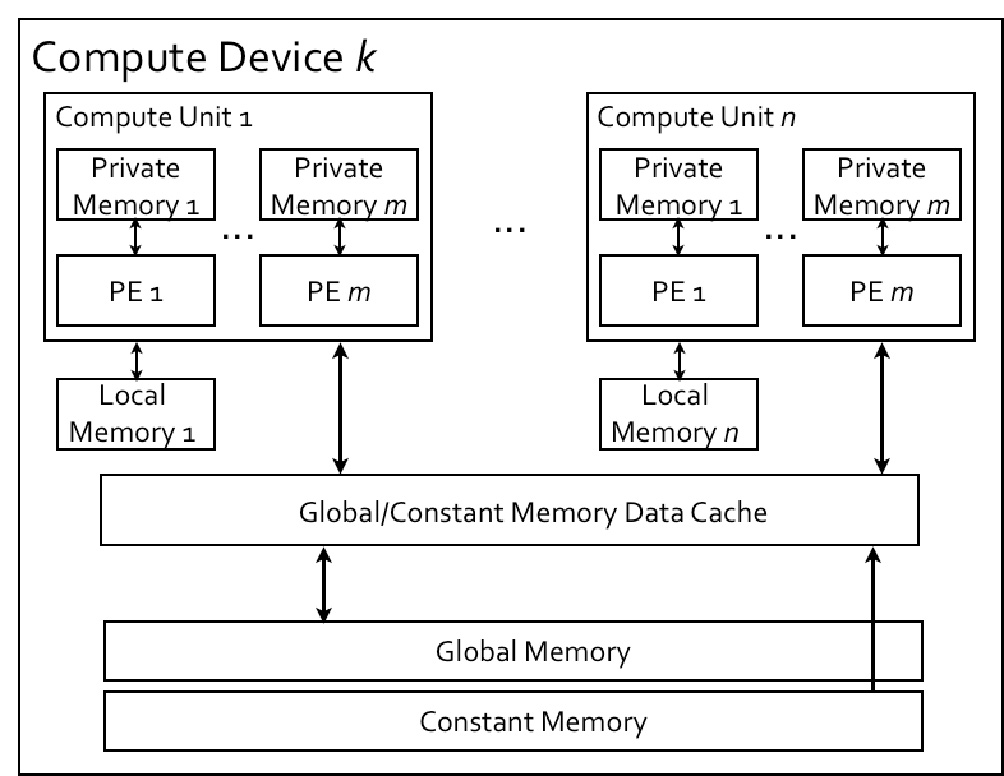
\includegraphics[width=0.73\textwidth]{figures/opencl-device.jpg} \\
 \end{center}
  {\tiny http://developer.amd.com/documentation/articles/PublishingImages/opencl\_figure5.jpg}
  \vspace{0.5cm}
\end{block}

\end{frame}




\begin{frame}[fragile]
\frametitle{OpenCL Kernel Language}

\begin{block}{Sample Operation: Inplace Vector Addition}
 \vspace*{-0.5cm}
 \begin{align*}
  \left(
  \begin{array}{c}
   x_1 \\
   x_2 \\
   \vdots \\
   x_n 
  \end{array} \right) +\!= 
  \left(
  \begin{array}{c}
   y_1 \\
   y_2 \\
   \vdots \\
   y_n 
  \end{array} \right)
 \end{align*}
\end{block}

 \vspace*{-0.3cm}
\begin{block}{OpenCL Kernel}
\begin{lstlisting}
__kernel void inplace_add(
          __global const float * vec1,
          __global const float * vec2,
          unsigned int size) 
{ 
  for (unsigned int i  = get_global_id(0); 
                    i  < size; 
                    i += get_global_size(0))
    x[i] += y[i];
}
\end{lstlisting}
\end{block}
\end{frame}




\begin{frame}[fragile]{OpenCL Kernel Language}

 \begin{block}{Just Like C}
  \begin{itemize}
   \item Datatypes: \lstinline|float|, \lstinline|double|, \lstinline|long|, ... , \lstinline|float2|, \lstinline|float4|, ...
   \item Keywords: \lstinline|for|, \lstinline|if|, \lstinline|switch|, ...
   \item ...
  \end{itemize}
 \end{block}

 \begin{block}{Thread Management}
  \begin{itemize}
   \item ID: \lstinline|get_local_id(dim)|, \lstinline|get_global_id(dim)|
   \item Count: \lstinline|get_local_size(dim)|, \lstinline|get_global_size(dim)|
   \item Sync: \lstinline|barrier(flags)|, \lstinline|mem_fence(flags)|
  \end{itemize}
 \end{block}

 \begin{block}{Memory Qualifiers}
  \begin{itemize}
   \item \lstinline|__global|: Global memory (e.g.~GPU RAM)
   \item \lstinline|__constant|: Constant global memory (vendor-specific!)
   \item \lstinline|__local|: Shared memory (per workgroup)
  \end{itemize}
 \end{block}

\end{frame}




\begin{frame}[fragile]{OpenCL Kernel Language}
  \begin{block}{Vector Assignment (Copy) Kernel}
    \begin{itemize}
     \item $x \Leftarrow y$ for (large) vectors $x$, $y$
    \end{itemize}
  \end{block}

  \only<1>{\vspace*{4.22cm}}
  \only<2>{\begin{center} \vspace*{0.84cm} 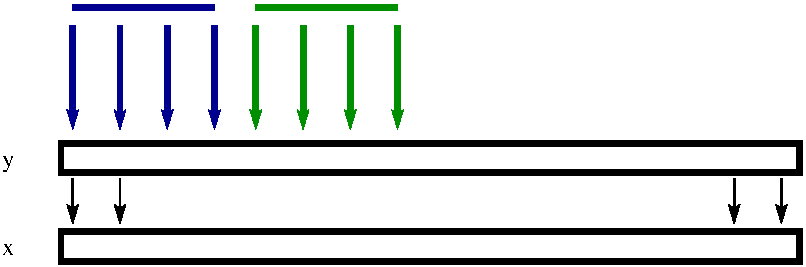
\includegraphics[width=0.8\textwidth]{figures/copy-kernel-gpu-1} \end{center}}
  \only<3>{\begin{center} \vspace*{0.85cm} 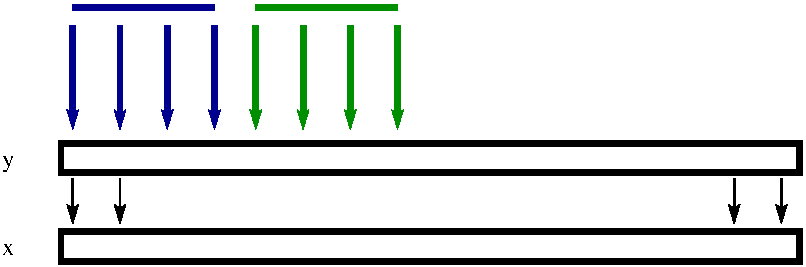
\includegraphics[width=0.8\textwidth]{figures/copy-kernel-gpu-1} \end{center}}
  \only<4>{\begin{center}                  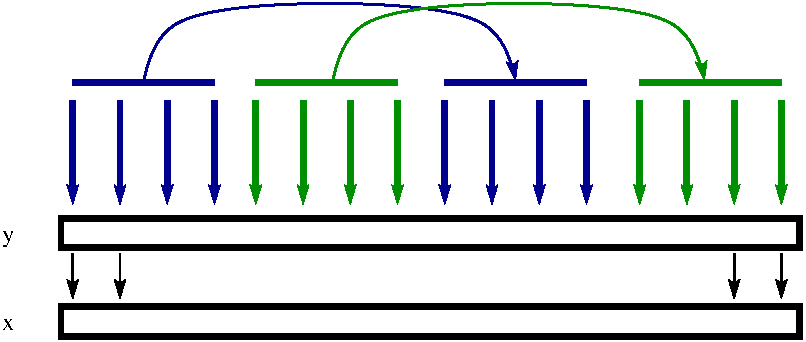
\includegraphics[width=0.8\textwidth]{figures/copy-kernel-gpu-full} \end{center}}
  
  \only<1>{\vspace*{2.52cm}}
  \only<2>{\vspace*{2.52cm}}
  \only<3>{
  \begin{block}{Parameters ($\gg 1000$ variations possible) }
   \begin{itemize}
    \item Local work size, global work size
    \item Vector types (float1, float2, ... , float16)
    \item Thread increment type
   \end{itemize}
  \end{block}}
  
  \only<4>{
  \begin{block}{Parameters ($\gg 1000$ variations possible) }
   \begin{itemize}
     \item \texttt{for (size\_t i = get\_global\_id(0); i < N;}
     \item \texttt{\ \ \ \ \ \ \ \ \ \ \ \ i+= get\_global\_size(0))}
     \item \texttt{\ \ x[i] = y[i];}
   \end{itemize}
  \end{block}
  }

\end{frame}


\begin{frame}{OpenCL Kernel Language}

  \begin{block}{No Synchronization: Vector Addition}
   \begin{center} 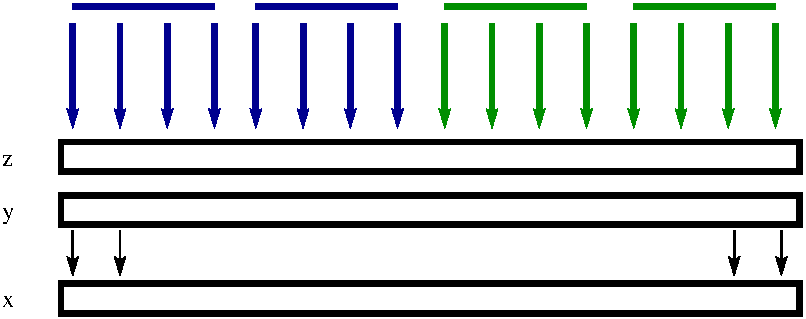
\includegraphics[width=0.6\textwidth]{figures/addition-kernel} \end{center}
  \end{block}
  
  \begin{block}{Synchronization: Dot Product}
   \begin{center} 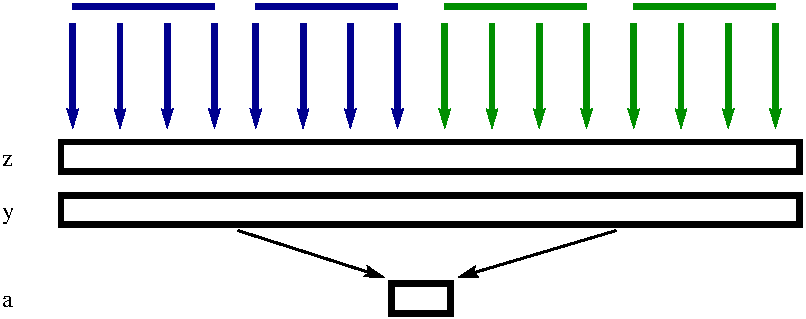
\includegraphics[width=0.6\textwidth]{figures/inner-product-kernel} \end{center}
  \end{block}

\end{frame}


